\documentclass[conference]{IEEEtran}
\IEEEoverridecommandlockouts

\usepackage{cite}
\usepackage{amsmath,amssymb,amsfonts,amsthm}
\usepackage{graphicx}
\usepackage{textcomp}
\usepackage{xcolor}
\usepackage{url}
\usepackage{tabularx}
\usepackage{tikz}
\usetikzlibrary{arrows.meta,positioning}
\usepackage{algorithm}
\usepackage{algpseudocode}
\usepackage{booktabs}
\usepackage{microtype}

\newtheorem{definition}{Definition}
\newtheorem{property}{Property}
\newtheorem{lemma}{Lemma}
\newtheorem{theorem}{Theorem}
\newtheorem{proposition}{Proposition}

% Shared TikZ styles for the structure diagrams
\tikzset{
  seg/.style={draw, rectangle, rounded corners=1pt, align=center,
              inner sep=2.5pt, font=\scriptsize},
  copynode/.style={seg, thick, fill=gray!12},
  prunednode/.style={seg, dashed},
  own/.style={-{Stealth[length=1.8mm]}},
  share/.style={-{Stealth[length=1.8mm]}, dashed},
}

\def\BibTeX{{\rm B\kern-.05em{\sc i\kern-.025em b}\kern-.08em
    T\kern-.1667em\lower.7ex\hbox{E}\kern-.125emX}}

\begin{document}

\title{Version-Aware Lazy Propagation for Partially Persistent Segment Trees:
Design, Correctness, and Differential Validation}

\author{\IEEEauthorblockN{Mohammad Nobinur}
\IEEEauthorblockA{\textit{Electrical \& Computer Engineering}\\
\textit{North South University}\\
Dhaka, Bangladesh\\
nobinur.251@northsouth.edu}
\and
\IEEEauthorblockN{Sunjare Zulfiker}
\IEEEauthorblockA{\textit{Electrical \& Computer Engineering}\\
\textit{North South University}\\
Dhaka, Bangladesh\\
sunjare.zulfiker.252@northsouth.edu}
\and
\IEEEauthorblockN{Ahsanur Rahman}
\IEEEauthorblockA{\textit{Electrical \& Computer Engineering}\\
\textit{North South University}\\
Dhaka, Bangladesh\\
ahsanur.rahman@northsouth.edu}
}

\maketitle

\begin{abstract}
Lazy segment trees support efficient range updates and range queries but overwrite their previous
state, while persistent structures retain historical access. Existing implementations already
combine persistence with generic lazy actions, so the contribution of this study is not the
combination itself. We isolate and analyze a specialized mechanism for partially persistent
range-add/range-sum trees: \emph{tag-retaining path copying}. A partially covered copied parent
retains its deferred addition, only update-intersecting children are copied, and its sum is
reconstructed by a node-local accounting rule. Historical queries carry inherited additions
without allocating or modifying nodes. We prove exact historical queries, immutability of every
published version, and update-frontier locality: each recursive update invocation appends one
node, and no disjoint segment is copied. This gives amortized $\mathcal{O}(\log n)$ update time,
worst-case $\mathcal{O}(\log n)$ query time, and at most $4(\lceil\log_2 n\rceil+1)$ copied nodes
per non-zero update. A C++17 implementation and two baseline implementations pass
67 deterministic tests. A sanitizer-checked differential campaign completed 180 seeded runs and
666{,}000 mixed operations with no oracle mismatch; all 353{,}102 updates satisfied the proved
allocation bound, and five selected structural cases matched their exact copy predictions. The
evidence supports functional and structural correctness within the tested domain; no empirical
wall-clock or memory-performance claim is made.
\end{abstract}

\begin{IEEEkeywords}
segment tree, lazy propagation, persistent data structure, partial persistence, range update,
historical query
\end{IEEEkeywords}

\section{Introduction}
\label{sec:intro}

Segment trees support logarithmic-time range queries by storing aggregate information over a
hierarchy of array intervals \cite{laaksonen2020guide}, following the general technique of
augmenting tree structures with aggregate data \cite{cormen2009introduction}. Lazy propagation
extends the structure to efficient range updates by deferring uniform changes at internal nodes
\cite{laaksonen2020guide}. A conventional lazy segment tree is ephemeral: each update mutates the
current tree, so earlier states cannot be queried after they are overwritten.

The ability to query earlier states is not merely of theoretical interest. Temporal graph
databases keep every historical state of an evolving graph queryable to answer audit and
provenance questions \cite{hou2024aeong}, and streaming analytics systems maintain
segment-tree-like structures over ever-growing time series so that any past time range can be
analyzed on demand \cite{qiu2024tucket}. Comparable needs arise in time-travel debugging, where
a runtime retains enough history to restore any earlier program state \cite{barr2014tardis}, and
in system-versioned relational tables, which keep superseded row versions precisely so that
later audit questions can be answered \cite{kulkarni2012temporal}; a typical question has the
form ``what was the sum over accounts $10$--$20$ as of version $5$?'' Answering such questions
efficiently requires a range-aggregate structure whose history is preserved, not overwritten.
These examples motivate historical access in general; they are analogies rather than evidence
that the exact range-add/range-sum interface studied here is deployed in those systems.

Persistence retains access to earlier states. Path copying creates a new root and copies only the
nodes affected by an update, while unchanged subtrees remain shared
\cite{driscoll1989persistent}. Immutability and structural sharing are also central to purely
functional persistent structures \cite{okasaki1998purely}. Combining these ideas with lazy
propagation requires care because destructive push-down would mutate nodes that may be reachable
from several historical roots. A direct copy-on-push adaptation can restore safety by copying
children before propagating a tag, but if the same mechanism is used during queries it allocates
on a logically read-only operation and may copy structure outside the queried frontier. The
design studied here instead avoids push-down in both updates and queries.

We study a focused operation model: range-add updates create a new version from the latest root,
while range-sum queries may inspect any published version. Two questions drive the analysis:
which node-local invariant supports push-free partial persistence for these operations, and
whether tag-retaining path copying preserves historical correctness while copying only the
update-intersecting frontier within logarithmic bounds. The invariant of
Section~\ref{sec:properties} answers the first, and the proofs of Section~\ref{sec:proofs}
answer the second. Deterministic, differential, and allocation-count checks
(Sections~\ref{sec:dataset} and~\ref{sec:result}) then corroborate the implementation against
an independent oracle and the proved allocation bound.

The paper makes the following contributions:

\begin{itemize}
  \item a precise partially persistent range-add/range-sum operation model with explicit
        publication and failure-isolation semantics;
  \item an immutable path-copying design whose node-local lazy invariant eliminates destructive
        push-down, together with correctness theorems showing that every historical query is
        answered exactly and that published versions are never modified;
  \item an update-frontier locality result showing that a non-zero update appends exactly one
        node per recursive invocation and never copies a disjoint segment, followed by the
        resulting logarithmic time and retained-space bounds; and
  \item a C++17 implementation of the proposed structure and two baseline implementations, together with
        67 deterministic cases, five exact structural measurements, and a seeded randomized
        differential campaign comprising 180 runs and 666{,}000 mixed operations
        (Section~\ref{sec:result}).
\end{itemize}

We make no first-use or generality claim for persistent lazy segment trees. In particular,
proconlib already documents a more general monoid/action interface, algebraic constraints,
logarithmic operation bounds, allocation-free queries, branching copies, and verified programs
\cite{proconlib2026persistent}; a contest editorial gives an earlier application-specific
construction \cite{orap2020unsquers}. The contribution evaluated here is
narrower and mechanism-specific: among the inspected sources, none jointly states the
tag-retaining invariant used here, proves that it excludes disjoint copies during updates, connects
that locality to historical-query correctness, and validates the resulting per-update allocation
bound. This specialization matters because retaining a parent tag can avoid copying disjoint
siblings merely to materialize inherited state. The comparisons in Section~\ref{sec:rel-work}
report only behavior verified in the cited papers, documentation, and pinned source revisions.

The remainder of the paper is organized as follows. Section~\ref{sec:rel-work} reviews related
work and positions our contribution. Section~\ref{sec:method} presents the operation model, the
persistent representation, the algorithms, the correctness theorems, and the complexity analysis.
Section~\ref{sec:dataset} presents the baseline implementations, validation methodology, and
synthetic inputs. Section~\ref{sec:result} reports the observed results and their interpretation,
Section~\ref{sec:limitations} discusses limitations and threats to validity, and
Section~\ref{sec:conclusion} concludes.

\section{Related Work}
\label{sec:rel-work}

\begin{table*}[!t]
\caption{Gap Analysis: Source-Reported Positioning of Key Prior Work}
\label{tab:sota}
\centering
\scriptsize
\renewcommand{\arraystretch}{1.18}
\setlength{\tabcolsep}{3.0pt}

\begin{tabular}{@{}p{2.6cm}p{2.5cm}p{2.7cm}p{2.7cm}p{5.9cm}@{}}
\toprule
\textbf{Work} &
\textbf{Lazy range tags} &
\textbf{Persistent history} &
\textbf{Range queries} &
\textbf{Gap relative to this study} \\
\midrule
Driscoll et al.\ 1989 \cite{driscoll1989persistent} &
$\times$ &
\checkmark\ (partial and full) &
n/a (generic structures) &
Founding persistence transformations (path copying, node copying) for linked structures; no
deferred range-update tags. \\

Okasaki 1998 \cite{okasaki1998purely} &
$\times$ &
\checkmark\ (functional immutability, sharing) &
n/a &
Persistence via immutability and structural sharing; lazy \emph{evaluation} schedules
computation and is not a deferred range-update tag. \\

Massri, seminar, n.d. \cite{massri_segment_trees} &
$\times$ &
\checkmark\ (persistent segment trees) &
\checkmark &
Persistent segment trees preserve node values across versions; no versioned lazy propagation. \\

Fiat and Kaplan 2003 \cite{fiat2003confluent} &
$\times$ &
\checkmark\ (confluent) &
n/a &
Version merging into version DAGs; orthogonal to deferred range-update tags. \\

Demaine et al.\ 2007 \cite{demaine2007retroactive} &
$\times$ &
\checkmark\ (retroactive) &
n/a &
Revising past operations is a different version model from querying past states. \\

Ibtehaz et al.\ 2021 \cite{ibtehaz2021multidimensional} &
\checkmark\ (multidimensional) &
$\times$ (ephemeral) &
\checkmark\ (latest state) &
Lazy range updates generalized to multiple dimensions; no historical versions. \\

Brodal et al.\ 2023 \cite{brodal2023external} &
$\times$ &
\checkmark\ (full, external memory) &
\checkmark\ (range reporting) &
I/O-optimized fully persistent search trees; range reporting rather than lazy-tagged range
aggregation. \\

Boneh et al.\ 2024 \cite{boneh2024string} &
\checkmark\ (parent-local invariant) &
$\times$ (ephemeral) &
\checkmark\ (zero reporting) &
Closest peer-reviewed lazy-invariant analogue (Lemma~35); no persistence and no range sums. \\

AeonG 2024 \cite{hou2024aeong} &
$\times$ &
\checkmark\ (anchor{+}delta graph history) &
$\times$ (graph queries) &
Temporal graph storage; no segment-tree range aggregates. \\

TUCKET 2024 \cite{qiu2024tucket} &
$\times$ &
\checkmark\ (append-only stream) &
\checkmark\ (approximate time ranges) &
Approximate factor analysis over an append-only stream segment tree; no independently versioned
exact range sums, no lazy tags. \\

\textbf{This study} &
\checkmark\ (\textbf{tag-retaining}) &
\checkmark\ (\textbf{partial}) &
\checkmark\ (\textbf{exact, allocation-free}) &
\textbf{Proved historical exactness and update-frontier copy locality; per-update allocation
bound validated (Sections~\ref{sec:method}--\ref{sec:result}).} \\
\bottomrule
\end{tabular}

\vspace{2pt}
\raggedright\footnotesize
\checkmark\ marks behavior the cited source reports; $\times$ marks behavior the cited source
does not address; n/a marks a criterion outside the source's operation model. Parenthetical
qualifiers restate the source's own scope. Each row describes only the cited source, not the
entire literature (Section~\ref{sec:scope}); the closest precedents are compared in
Section~\ref{sec:direct}.
\end{table*}

Table~\ref{tab:sota} positions the foundational and adjacent work inspected for this study
along three source-reported criteria---deferred range-update (lazy) tags, persistent history,
and range queries---and states the gap each line of work leaves relative to our operation
model. The entries describe only the cited sources and assert no universal absence
(Section~\ref{sec:scope}); the closest precedents, proconlib \cite{proconlib2026persistent} and
the UNSQUERS editorial \cite{orap2020unsquers}, are examined at the mechanism level in
Section~\ref{sec:direct}.

\subsection{Foundations and Adjacent Lazy Invariants}

Driscoll et al.\ define partial and full persistence and give generic transformations for linked
data structures, using search trees as a running example \cite{driscoll1989persistent}. Their
framework is substantially more general than point updates, but it does not specialize its
analysis to segment aggregates with deferred range actions. Sarnak and Tarjan provide a classical
application of persistent search trees to planar point location \cite{sarnak1986planar}, while
Okasaki develops persistence through functional immutability and structural sharing
\cite{okasaki1998purely}. Okasaki's lazy evaluation schedules computation; it is distinct from a
segment tree's deferred range-update tag.

Standard and persistent segment trees are described in textbook and seminar treatments
\cite{laaksonen2020guide,massri_segment_trees}. A peer-reviewed example of a specialized
node-local lazy invariant appears in Boneh et al.'s range-add/zero-reporting structure
\cite[Lemma~35]{boneh2024string}: local values maintain minimum/count information in an ephemeral
tree. This establishes that parent-local deferred accounting is not itself new; the present work
studies its interaction with immutable historical versions and range sums. More expansive version models
include confluent persistence, which merges versions \cite{fiat2003confluent}, retroactivity,
which revises past operations \cite{demaine2007retroactive}, and fully persistent search trees in
the external-memory model \cite{brodal2023external}. These are foundational or adjacent to the
latest-version-only in-memory model used here, not direct competitors.

Other work illustrates why the interaction between an aggregate structure and its update model
must be made explicit. Ibtehaz et al.\ redesign range updates for multidimensional segment trees
\cite{ibtehaz2021multidimensional}. AeonG retains graph history with anchors and deltas
\cite{hou2024aeong}, and TUCKET uses an append-only stream segment tree for approximate tensor
factor analysis over time ranges \cite{qiu2024tucket}. Neither system implements independently
versioned range-add/range-sum arrays, so they motivate temporal access but do not establish the
direct research gap.

\subsection{Direct Persistent-Lazy Precedents}
\label{sec:direct}

The closest inspected precedent is proconlib \cite{proconlib2026persistent}. Its documentation
specifies a monoid $S$, a composable mapping set $F$, distributivity constraints, copy-returning
updates on retained tree values, product queries, and $\mathcal{O}(\log n)$ bounds. Its
\texttt{prod} query is \texttt{const}, carries an inherited mapping through recursion, and appends
no nodes; two verification programs are linked. These features overlap substantially with the
present design and exceed it in genericity and version branching. The pinned source also reveals
a concrete mechanism-level difference. During a partial update it passes the accumulated mapping
to both children; a disjoint child is copied when that mapping is non-identity, thereby
materializing deferred state before the parent is rebuilt with an identity tag. The proposed
algorithm instead retains the copied parent's tag and never invokes the update on a disjoint
child. This is a locality distinction, not a claim of general superiority.

As a reproducible source trace, consider an eight-leaf tree to which a full-range addition is
applied, followed by an update of only the half-open interval $[3,4)$ (the inclusive interval
$[3,3]$ in our notation). Lines
159--177 of the pinned proconlib implementation append seven nodes: four on the intersecting
root-to-leaf path and three disjoint nodes that receive the inherited mapping. Algorithm
\ref{alg:update} appends the four intersecting path nodes. The example isolates retained-tag copy
locality; it is an analytical trace of the two sources, not a timing or memory benchmark.

The UNSQUERS editorial gives an earlier specialized construction for persistent range updates and
historical range maxima \cite{orap2020unsquers}. It explains the application and total asymptotic
cost, but its query calls a push routine that allocates child copies and mutates nodes. No separate
correctness proof, failure contract, or systematic validation campaign is reported. It is useful
as evidence of engineering practice, not as a formally analyzed equivalent of our operation
model.

\subsection{Search Scope and Gap Synthesis}
\label{sec:scope}

To keep the gap claim bounded, the literature check used exact-phrase web searches for
``persistent lazy segment tree'' and ``persistent segment tree with lazy propagation,'' a combined
search for persistent segment trees, lazy propagation, and range updates, and site-limited queries
over arXiv and DOI-indexed records; sources were inspected through Aug.~3, 2026. Table
\ref{tab:sota} positions the foundational and adjacent sources located in that process, and
Section~\ref{sec:direct} examines the direct engineering precedents. Neither establishes
universal absence.

The gap is therefore not the existence of persistent lazy propagation, generic actions,
allocation-free historical queries, or logarithmic complexity---proconlib already supplies all
four. The contribution is the narrower conjunction of (i) a tag-retaining range-add/range-sum
invariant, (ii) a proof that only the intersecting update frontier is copied while old versions
remain exact, and (iii) implementation-level differential and per-update allocation validation.
The specialization sacrifices proconlib's generality and branching updates, but makes the copy
mechanism and its obligations explicit enough to prove and measure directly.

\section{Methodology}
\label{sec:method}

We first fix the operation model and the invariants that govern the persistent representation,
then derive the update and query algorithms from those invariants, prove their correctness and
complexity, and validate the implementation against independent baseline implementations
through deterministic tests, randomized differential testing, and exact node-count checks
(Section~\ref{sec:dataset}).

\subsection{Operation Model and Definitions}
\label{sec:def}

Let the initial array be
\[
A^{(0)} = \langle a_0, a_1, \ldots, a_{n-1} \rangle ,
\]
where indices are zero-based and every range is inclusive.

\begin{definition}[Range-add update]
\label{def:update}
Given the latest version $A^{(t)}$, indices $0 \leq l \leq r < n$, and a value $\Delta$, the
operation creates version $A^{(t+1)}$ such that
\[
A^{(t+1)}_i =
\begin{cases}
A^{(t)}_i + \Delta, & l \leq i \leq r,\\
A^{(t)}_i, & \text{otherwise}.
\end{cases}
\]
Updates from versions older than $t$ are outside the operation model.
\end{definition}

A version is \emph{published} once its root has been recorded by initialization or by a
successful update; a failed operation publishes nothing
(Section~\ref{sec:properties}).

\begin{definition}[Historical range-sum query]
\label{def:query}
For any published version $v$ and interval $[l,r]$ with $0 \leq l \leq r < n$, the query
returns
\[
\operatorname{sum}(v,l,r) = \sum_{i=l}^{r} A^{(v)}_i .
\]
The query does not create a version and does not modify stored state.
\end{definition}

\begin{definition}[Partial persistence]
\label{def:persistence}
A version sequence is partially persistent when every published version can be queried while
only the latest version can serve as the base of an update \cite{driscoll1989persistent}.
\end{definition}

All array values, lazy values, segment lengths, products, and sums use signed 64-bit storage and
are required to remain representable by that type. Accordingly, the mathematical model assumes
$1 \leq n \leq \texttt{LLONG\_MAX}$; the implementation additionally assumes that $2n-1$ is
representable by \texttt{size\_t} and that the required storage can be allocated. Full
persistence, range assignment, and aggregate operations other than sum are not considered.

\subsection{Persistent Representation}
\label{sec:representation}

The proposed \texttt{PersistentLazySegmentTree} owns an append-only node \emph{arena} and a
root-index table. Each node stores left and right child indices, a local segment sum that includes
its own lazy value but excludes proper-ancestor lazy values, and a lazy-add value:
\[
\textit{node} = (\textit{left}, \textit{right}, \textit{sum}, \textit{lazy}).
\]
In the reference implementation these are four nominally 8-byte fields (two arena indices and two
signed 64-bit values). A 32-byte node is therefore an observation for the inspected ABI, not a
portable C++ language guarantee; the structural evaluation uses node counts rather than assuming
a portable byte size.
Version $v$'s tree is reached through $\textit{roots}[v]$, the arena index of its root. Arena
indices remain stable across vector reallocations, and unchanged children are shared across
versions. Sharing is physical: two versions share a subtree exactly when their trees store the
same arena index. A default-constructed structure has no versions. Initialization with
$n \geq 1$ creates version 0 with $2n-1$ nodes and all lazy values zero; initialization with
$n = 0$ is also permitted and publishes a version 0 with no nodes, on which every range
operation fails validation because no indices satisfy $0 \leq l \leq r < n$. The remainder of
the paper therefore assumes $n \geq 1$. Every successful range update starts from the latest root
and returns the new version identifier. Historical queries select a root by version identifier.

\subsection{Design Invariants}
\label{sec:properties}

The persistent structure is governed by the following properties, maintained for every node
reachable from every published root.

\begin{property}[Published-node immutability]
\label{prop:immutable}
Once a root is published, no node reachable from that root is modified.
\end{property}

\begin{property}[Version publication]
\label{prop:publication}
Each successful update creates exactly one sequential version from the latest root. A failed
operation publishes no root and leaves all previous versions unchanged.
\end{property}

\begin{property}[Read-only historical queries]
\label{prop:readonly}
A query allocates no tree nodes, publishes no version, and mutates no stored state.
\end{property}

\begin{property}[Lazy contribution]
\label{prop:lazy}
For a node covering a segment of length $m$, the stored sum includes the node's own lazy
addition, while the child sums do not. An internal node therefore satisfies
\[
\textit{sum}
= \textit{left.sum} + \textit{right.sum} + m \cdot \textit{lazy}.
\]
For a leaf ($m = 1$) the same convention applies with no child terms: a leaf's stored sum
already includes the leaf's own lazy value.
\end{property}

\begin{property}[Exact representation]
\label{prop:exact}
For every published version $v$ and every node $x$ reachable from $\textit{roots}[v]$ covering
segment $I_x$,
\[
x.\textit{sum} \;=\; \sum_{i \in I_x} A^{(v)}_i \;-\; |I_x| \cdot \Lambda_v(x),
\]
where $\Lambda_v(x)$ denotes the sum of the lazy values held by the proper ancestors of $x$ in
the tree of version $v$.
\end{property}

Property~\ref{prop:lazy} is the central convention of the design: every deferred contribution is
stored exactly once, either inside a node's own sum or in an ancestor's lazy value pending
inheritance. It permits partial updates without pushing a node's lazy value into children that may
be shared with older versions, and---in contrast to a copy-on-push variant, which must duplicate
both children whenever a tag is pushed---it keeps historical queries allocation-free
(Property~\ref{prop:readonly}).

\subsection{Persistent Range Update}
\label{sec:update}

Algorithm~\ref{alg:update} shows the update. For full coverage, it appends a copy of the current
node, increases its sum by $\Delta m$, and increases its lazy value by $\Delta$, where $m$ is the
segment length. For partial coverage, it recursively copies only update-intersecting child paths;
unchanged children keep their existing arena indices. The copied parent retains its own lazy
value and recomputes its sum by the rule of Property~\ref{prop:lazy}. No destructive push-down is
needed. The new root is published only after the recursive update completes. A zero-delta update
creates a version by sharing the latest root and allocates no nodes; distinct version
identifiers may therefore denote identical array states, so the version count bounds, but need
not equal, the number of distinct states.

\begin{algorithm}[!t]
\caption{Persistent range-add update}
\label{alg:update}
\begin{algorithmic}[1]
\Procedure{RangeAdd}{$l, r, \Delta$}
  \State validate that a version exists and $0 \leq l \leq r < n$
  \State $V \gets$ latest version identifier
  \If{$\Delta = 0$} \Comment{fast path: share the latest root}
    \State append $\textit{roots}[V]$ to $\textit{roots}$; \Return $V+1$
  \EndIf
  \State $c \gets |\textit{nodes}|$ \Comment{arena checkpoint}
  \State \textbf{try:} $\rho \gets \Call{Update}{\textit{roots}[V], 0, n-1, l, r, \Delta}$
  \State \hspace{1.5em} append $\rho$ to $\textit{roots}$
  \State \textbf{on allocation failure in either step:} truncate $\textit{nodes}$ to $c$;
         publish nothing; re-signal the failure
  \State \Return $V+1$ \Comment{reached only on success}
\EndProcedure
\Statex
\Function{Update}{$x, s, e, l, r, \Delta$} \Comment{node $x$ covers $[s,e]$}
  \State $m \gets e - s + 1$
  \State $y \gets$ a local copy of node $x$
  \If{$l \leq s$ \textbf{and} $e \leq r$} \Comment{full coverage}
    \State $y.\textit{sum} \gets y.\textit{sum} + \Delta \cdot m$
    \State $y.\textit{lazy} \gets y.\textit{lazy} + \Delta$
    \State \Return \Call{Append}{$y$} \Comment{children stay shared}
  \EndIf
  \State $\mu \gets \lfloor (s+e)/2 \rfloor$ \Comment{partial coverage}
  \If{$l \leq \mu$}
    \State $y.\textit{left} \gets \Call{Update}{x.\textit{left}, s, \mu, l, r, \Delta}$
  \EndIf
  \If{$r > \mu$}
    \State $y.\textit{right} \gets \Call{Update}{x.\textit{right}, \mu+1, e, l, r, \Delta}$
  \EndIf
  \State $y.\textit{sum} \gets y.\textit{left}.\textit{sum} + y.\textit{right}.\textit{sum}
          + y.\textit{lazy} \cdot m$
  \State \Return \Call{Append}{$y$}
\EndFunction
\end{algorithmic}
\end{algorithm}

\begin{proposition}[Update-frontier locality]
\label{prop:frontier}
For every successful non-zero range update, each invocation of \textsc{Update} covers a segment
that intersects the update interval, appends exactly one copied node, and causes no other node
append. Consequently, no disjoint segment is copied.
\end{proposition}

\begin{proof}
The initial call covers the validated update interval. A recursive child call occurs only under
$l\leq\mu$ or $r>\mu$, precisely the conditions that the corresponding child intersects
$[l,r]$; thus the intersection property holds inductively. A full-coverage call appends once and
returns. A partial-coverage call recursively obtains any changed child indices and then appends
its single rebuilt parent. No other statement in \textsc{Update} appends a node. Therefore the
calls and appended nodes are in one-to-one correspondence, and disjoint children retain their old
indices without being invoked or copied.
\end{proof}

Fig.~\ref{fig:pathcopy} illustrates the resulting version structure on the reference example
$A^{(0)} = \langle 1, 2, 3, 4 \rangle$: a full-coverage update copies only the root, a partial
update copies one path per affected side, and every untouched subtree is shared with older
versions. No arrow ever points from an old node to a new one, which is the graph form of
Property~\ref{prop:immutable}.

\begin{figure*}[!t]
\centering
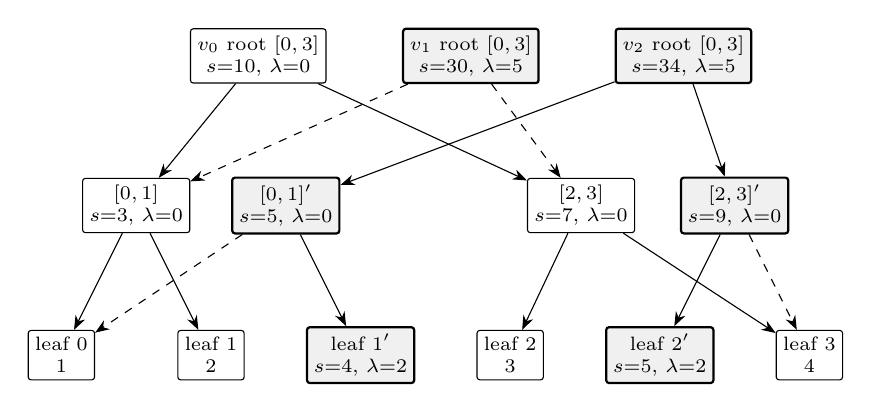
\begin{tikzpicture}
  % leaves
  \node[seg]      (l0)  at (0,0)    {leaf $0$\\ $1$};
  \node[seg]      (l1)  at (1.9,0)  {leaf $1$\\ $2$};
  \node[copynode] (l1c) at (3.8,0)  {leaf $1'$\\ $s{=}4$, $\lambda{=}2$};
  \node[seg]      (l2)  at (5.7,0)  {leaf $2$\\ $3$};
  \node[copynode] (l2c) at (7.6,0)  {leaf $2'$\\ $s{=}5$, $\lambda{=}2$};
  \node[seg]      (l3)  at (9.5,0)  {leaf $3$\\ $4$};
  % internal nodes
  \node[seg]      (A)  at (0.95,1.9) {$[0,1]$\\ $s{=}3$, $\lambda{=}0$};
  \node[copynode] (A2) at (2.85,1.9) {$[0,1]'$\\ $s{=}5$, $\lambda{=}0$};
  \node[seg]      (B)  at (6.6,1.9)  {$[2,3]$\\ $s{=}7$, $\lambda{=}0$};
  \node[copynode] (B2) at (8.55,1.9) {$[2,3]'$\\ $s{=}9$, $\lambda{=}0$};
  % roots
  \node[seg]      (r0) at (2.5,3.8) {$v_0$ root $[0,3]$\\ $s{=}10$, $\lambda{=}0$};
  \node[copynode] (r1) at (5.2,3.8) {$v_1$ root $[0,3]$\\ $s{=}30$, $\lambda{=}5$};
  \node[copynode] (r2) at (7.9,3.8) {$v_2$ root $[0,3]$\\ $s{=}34$, $\lambda{=}5$};
  % edges
  \draw[own]   (r0) -- (A);
  \draw[own]   (r0) -- (B);
  \draw[share] (r1) -- (A);
  \draw[share] (r1) -- (B);
  \draw[own]   (r2) -- (A2);
  \draw[own]   (r2) -- (B2);
  \draw[own]   (A)  -- (l0);
  \draw[own]   (A)  -- (l1);
  \draw[share] (A2) -- (l0);
  \draw[own]   (A2) -- (l1c);
  \draw[own]   (B)  -- (l2);
  \draw[own]   (B)  -- (l3);
  \draw[own]   (B2) -- (l2c);
  \draw[share] (B2) -- (l3);
\end{tikzpicture}
\caption{Path copying with structural sharing for $A^{(0)} = \langle 1,2,3,4 \rangle$. Version
$v_1 = \textsc{RangeAdd}(0,3,5)$ fully covers the root, so it copies only the root (sum
$10+5\cdot4=30$, lazy $5$) and shares both subtrees of $v_0$ (dashed arrows). Version
$v_2 = \textsc{RangeAdd}(1,2,2)$ partially covers both halves, so it copies one path per side and
recomputes each parent by Property~\ref{prop:lazy}, e.g., the $v_2$ root stores
$5+9+5\cdot4=34$. Shaded nodes are copies appended by updates; $s$ denotes the stored sum,
$\lambda$ the stored lazy value, and lazy values not shown are zero. The copied leaves receive
$\lambda{=}2$ from the full-coverage branch of Algorithm~\ref{alg:update}; by
Property~\ref{prop:lazy} a leaf's stored sum already includes its own lazy value. No arrow
points from an old node to a new one.}
\label{fig:pathcopy}
\end{figure*}

The update recursion visits at most four nodes per level---the standard segment-tree boundary
argument---and appends one copy per visited node. Fig.~\ref{fig:frontier} shows the visited
frontier of a worst-case update shape on $n=8$: seven copies in total, never more than four on a
level, while every skipped subtree is shared unchanged.

\begin{figure}[!t]
\centering
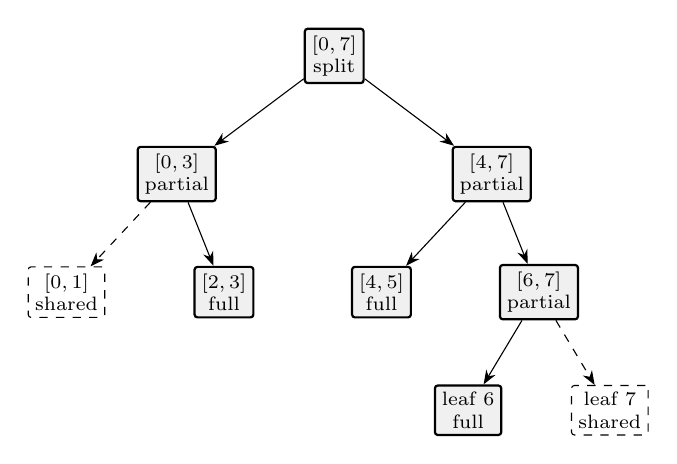
\begin{tikzpicture}
  \node[copynode]   (R)  at (3.9,4.5) {$[0,7]$\\ split};
  \node[copynode]   (L1) at (1.9,3.0) {$[0,3]$\\ partial};
  \node[copynode]   (R1) at (5.9,3.0) {$[4,7]$\\ partial};
  \node[prunednode] (s1) at (0.5,1.5) {$[0,1]$\\ shared};
  \node[copynode]   (L2) at (2.5,1.5) {$[2,3]$\\ full};
  \node[copynode]   (R2) at (4.5,1.5) {$[4,5]$\\ full};
  \node[copynode]   (R3) at (6.5,1.5) {$[6,7]$\\ partial};
  \node[copynode]   (l6) at (5.6,0)   {leaf $6$\\ full};
  \node[prunednode] (s2) at (7.4,0)   {leaf $7$\\ shared};
  \draw[own]   (R)  -- (L1);
  \draw[own]   (R)  -- (R1);
  \draw[share] (L1) -- (s1);
  \draw[own]   (L1) -- (L2);
  \draw[own]   (R1) -- (R2);
  \draw[own]   (R1) -- (R3);
  \draw[own]   (R3) -- (l6);
  \draw[share] (R3) -- (s2);
\end{tikzpicture}
\caption{Visited frontier of $\textsc{RangeAdd}(2,6,\Delta)$ on $n=8$: seven nodes are copied
(shaded), never more than four per level. Dashed nodes are skipped subtrees that remain shared
with the previous version.}
\label{fig:frontier}
\end{figure}

\subsection{Historical Range Query}
\label{sec:query}

Algorithm~\ref{alg:query} shows the query. It carries an \emph{inherited} lazy value $\Lambda$,
the sum of lazy values on the path strictly above the current node. For a fully covered node of
length $m$, it returns $\textit{sum} + m \cdot \Lambda$. For partial coverage, it passes
$\Lambda + \textit{lazy}$ to both recursive calls, moving the node's own lazy value from the node
into the accumulator. The node's own lazy value is not added again on full coverage because, by
Property~\ref{prop:lazy}, it is already included in the stored sum. The query therefore counts
every deferred addition exactly once while allocating and mutating nothing
(Property~\ref{prop:readonly}).

\begin{algorithm}[!t]
\caption{Historical range-sum query}
\label{alg:query}
\begin{algorithmic}[1]
\Procedure{RangeSum}{$v, l, r$}
  \State validate version $v$ and $0 \leq l \leq r < n$
  \State \Return \Call{Query}{$\textit{roots}[v], 0, n-1, l, r, 0$}
\EndProcedure
\Statex
\Function{Query}{$x, s, e, l, r, \Lambda$} \Comment{node $x$ covers $[s,e]$}
  \If{$r < s$ \textbf{or} $e < l$} \Return $0$ \Comment{disjoint}
  \EndIf
  \If{$l \leq s$ \textbf{and} $e \leq r$} \Comment{full coverage}
    \State \Return $x.\textit{sum} + \Lambda \cdot (e - s + 1)$
  \EndIf
  \State $\mu \gets \lfloor (s+e)/2 \rfloor$;\;
         $\Lambda' \gets \Lambda + x.\textit{lazy}$
  \State $L \gets \Call{Query}{x.\textit{left}, s, \mu, l, r, \Lambda'}$
  \State $R \gets \Call{Query}{x.\textit{right}, \mu+1, e, l, r, \Lambda'}$
  \State \Return $L + R$
\EndFunction
\end{algorithmic}
\end{algorithm}

Fig.~\ref{fig:query} traces $\operatorname{sum}(v_2, 1, 2)$ on the example of
Fig.~\ref{fig:pathcopy}. The root's deferred $5$ reaches each selected leaf exactly once through
the accumulator, and disjoint subtrees are pruned; the returned value is $9 + 10 = 19$, matching
the hand-traced expectation.

\begin{figure}[!t]
\centering
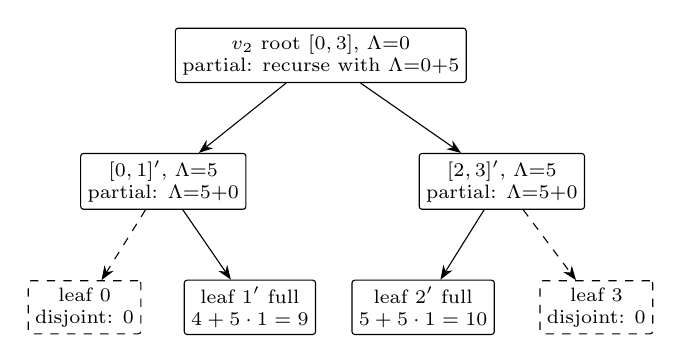
\begin{tikzpicture}
  \node[seg] (q0) at (3.6,3.2)
    {$v_2$ root $[0,3]$, $\Lambda{=}0$\\ partial: recurse with $\Lambda{=}0{+}5$};
  \node[seg] (qa) at (1.6,1.6)
    {$[0,1]'$, $\Lambda{=}5$\\ partial: $\Lambda{=}5{+}0$};
  \node[seg] (qb) at (5.9,1.6)
    {$[2,3]'$, $\Lambda{=}5$\\ partial: $\Lambda{=}5{+}0$};
  \node[prunednode] (d0) at (0.6,0)  {leaf $0$\\ disjoint: $0$};
  \node[seg]        (s1) at (2.7,0)  {leaf $1'$ full\\ $4+5\cdot1=9$};
  \node[seg]        (s2) at (4.9,0)  {leaf $2'$ full\\ $5+5\cdot1=10$};
  \node[prunednode] (d3) at (7.1,0)  {leaf $3$\\ disjoint: $0$};
  \draw[own]   (q0) -- (qa);
  \draw[own]   (q0) -- (qb);
  \draw[share] (qa) -- (d0);
  \draw[own]   (qa) -- (s1);
  \draw[own]   (qb) -- (s2);
  \draw[share] (qb) -- (d3);
\end{tikzpicture}
\caption{Descent of $\operatorname{sum}(v_2,1,2)$ on the example of Fig.~\ref{fig:pathcopy} with
the inherited-lazy accumulator $\Lambda$. The root's deferred $5$ reaches each selected leaf
exactly once; dashed nodes are pruned as disjoint. The copied leaves' own lazy values
($\lambda{=}2$) are already contained in their stored sums and are not added again on full
coverage. The result is $9+10=19$.}
\label{fig:query}
\end{figure}

\subsection{Validation and Failure Isolation}
\label{sec:failure}

Version and range validation occurs before node allocation, so---under the no-overflow assumption
above---the remaining failure considered by the implementation is memory allocation while
appending nodes or a root. An update records an arena checkpoint, rolls back appended nodes if an
exception occurs, and publishes a root only after the recursive update completes
(Algorithm~\ref{alg:update}). Initialization builds replacement state separately and swaps it into
the object only after the complete build succeeds. This argument relies on the standard
exception guarantees of \texttt{std::vector} and on non-throwing copies of the node's integral
fields. The deterministic suite tests validation-error isolation; allocation failure has not been
fault-injected, so that part is a code-level guarantee rather than an empirical result.

\subsection{Correctness Guarantees}
\label{sec:proofs}

We now show that the algorithms establish and maintain the invariants of
Section~\ref{sec:properties}. All proofs are by induction on segment length and, for
Theorem~\ref{thm:correct}, additionally on the update sequence. Where a proof applies
Properties~\ref{prop:lazy} and~\ref{prop:exact} to a tree still under construction during an
update, $\Lambda_v(x)$ is read as the sum of lazy values on the path strictly above $x$ within
the tree under consideration.

\begin{lemma}[Build correctness]
\label{lem:build}
After initialization with $n \geq 1$, the tree rooted at $\textit{roots}[0]$ satisfies
Properties~\ref{prop:lazy} and~\ref{prop:exact} for $A^{(0)}$, and every lazy value is zero.
\end{lemma}

\begin{proof}
By induction on segment length. A leaf stores its array value and a zero lazy value, so its
stored sum is exact. An internal node covering a segment of length $m$ stores the sum of two
correct children plus $m \cdot 0$, so Property~\ref{prop:lazy} holds; and because every lazy
value on the path above any node is zero, $\Lambda_0(x) = 0$ for all $x$ and the stored sum
equals the true segment sum, establishing Property~\ref{prop:exact}.
\end{proof}

\begin{lemma}[Update preservation]
\label{lem:update}
Consider a call $\operatorname{Update}(x,s,e,l,r,\Delta)$ reached under a proper-ancestor lazy sum
$\Gamma$. Suppose $x$ covers $I=[s,e]$, satisfies Property~\ref{prop:lazy}, and
$x.\textit{sum}=\sum_{i\in I}A_i-|I|\Gamma$. Let $A'$ be obtained by adding $\Delta$ on
$I\cap[l,r]$. Then:
\begin{enumerate}
  \item the returned node $x'$ satisfies Property~\ref{prop:lazy} and
        $x'.\textit{sum}=\sum_{i\in I}A'_i-|I|\Gamma$, and every descendant of $x'$ satisfies
        the analogous equation under its new proper-ancestor lazy sum;
  \item every old node is unchanged; and
  \item each untouched subtree remains shared.
\end{enumerate}
\end{lemma}

\begin{proof}
By induction on $I=[s,e]$, with $m=|I|$. \emph{Full coverage}: the copy $y$ stores
$y.\textit{sum}=x.\textit{sum}+m\Delta$ and
$y.\textit{lazy}=x.\textit{lazy}+\Delta$. Because every element of $I$ increases by $\Delta$,
\[
y.\textit{sum}
=\sum_{i\in I}A_i-m\Gamma+m\Delta
=\sum_{i\in I}A'_i-m\Gamma.
\]
Both children remain unchanged. Increasing the parent lazy value and its stored sum by the same
$m\Delta$ preserves Property~\ref{prop:lazy}, so the new contribution is represented at $y$
without entering either child. For every shared descendant $z$, both its logical segment sum and
the subtracted proper-ancestor contribution increase by $|I_z|\Delta$; hence the changes cancel
in Property~\ref{prop:exact}, and $z$'s unchanged stored sum remains valid.

\emph{Partial coverage}: the copied node $y$ retains
$y.\textit{lazy}=x.\textit{lazy}$. A child $c$ is reached under proper-ancestor sum
$\Gamma_c=\Gamma+y.\textit{lazy}$. The inductive hypothesis applies to each intersecting child;
a disjoint child already satisfies the same equation because its logical values are unchanged.
Writing $I_L$ and $I_R$ for the child segments, recomputation gives
\begin{align*}
y.\textit{sum}
&=\sum_{i\in I_L}A'_i-|I_L|\Gamma_c\\
&\quad+\sum_{i\in I_R}A'_i-|I_R|\Gamma_c\\
&\quad+m\,y.\textit{lazy}\\
&=\sum_{i\in I}A'_i-m\Gamma.
\end{align*}
Thus both required properties hold in either case. The algorithm appends new nodes and never
assigns to an existing arena element, so old nodes remain unchanged and disjoint subtrees retain
their original indices.
\end{proof}

\begin{lemma}[Single counting]
\label{lem:query}
For a tree satisfying Properties~\ref{prop:lazy} and~\ref{prop:exact},
$\operatorname{Query}(x, s, e, l, r, \Lambda)$ returns the exact sum of the represented values over
$[s,e] \cap [l,r]$, where $\Lambda$ is the sum of lazy values on the path strictly above $x$.
\end{lemma}

\begin{proof}
By induction on the segment $[s,e]$ with $m = e - s + 1$. \emph{Disjoint}
($[s,e] \cap [l,r] = \emptyset$): the call returns $0$, which is exact. \emph{Full coverage}
($[s,e] \subseteq [l,r]$): the call returns $x.\textit{sum} + \Lambda \cdot m$. By
Property~\ref{prop:exact}, $x.\textit{sum}$ equals the true segment sum minus
$m \cdot \Lambda_v(x)$, and by assumption $\Lambda = \Lambda_v(x)$, so the returned value equals
the true segment sum: every lazy value stored at $x$ or below is counted exactly once inside
$x.\textit{sum}$, and every ancestor lazy value exactly once through $\Lambda$.
\emph{Partial coverage}: the call recurses on both children with accumulator
$\Lambda + x.\textit{lazy}$. For each child $c$, the proper-ancestor tag sum is
$\Lambda_v(c) = \Lambda_v(x) + x.\textit{lazy}$, so the inductive hypothesis applies to each
child; the child segments partition $[s,e]$, so summing the two results counts each element of
$[s,e] \cap [l,r]$ exactly once, and no contribution is dropped or duplicated.
\end{proof}

\begin{theorem}[Historical query correctness]
\label{thm:correct}
For every published version $v$ and valid range $[l,r]$,
$\operatorname{sum}(v, l, r) = \sum_{i=l}^{r} A^{(v)}_i$.
\end{theorem}

\begin{proof}
Lemma~\ref{lem:build} establishes Properties~\ref{prop:lazy} and~\ref{prop:exact} for version 0.
Lemma~\ref{lem:update} extends them to each later version by induction over the update sequence,
and Properties~\ref{prop:immutable} and~\ref{prop:publication} guarantee that later operations
cannot invalidate them: updates only append nodes, and failed operations roll back to a
checkpoint before publication. Applying Lemma~\ref{lem:query} at $\textit{roots}[v]$ with
$\Lambda = 0$---the root has no proper ancestors---yields the stated sum.
\end{proof}

\begin{theorem}[Partial persistence]
\label{thm:persist}
Every successful range-add publishes exactly one new version derived from the latest version, all
earlier versions remain queryable with unchanged results, and unchanged subtrees are physically
shared between versions.
\end{theorem}

\begin{proof}
$\textsc{RangeAdd}$ appends exactly one entry to \textit{roots} per successful call and passes
only the latest root to $\textsc{Update}$, so each version derives from its immediate
predecessor (Definition~\ref{def:persistence}). By Lemma~\ref{lem:update}, $\textsc{Update}$
writes only newly appended nodes, so no node reachable from an earlier root is modified, and by
Theorem~\ref{thm:correct} earlier query results are unchanged. Untouched subtrees are physically
shared because the copied parent stores the same child arena indices as the original. A
zero-delta update appends only a root entry aliasing the latest root, and a failed operation
truncates the arena to its checkpoint and publishes nothing, leaving the arena prefix, the root
table, and all version counts unchanged.
\end{proof}

\subsection{Complexity Analysis}
\label{sec:complexity}

\begin{table}[!t]
\caption{Time and Space Bounds of the Proposed Structure}
\label{tab:complexity}
\centering
\footnotesize
\renewcommand{\arraystretch}{1.25}
\begin{tabularx}{\columnwidth}{@{}p{2.7cm}p{2.1cm}X@{}}
\toprule
\textbf{Operation} & \textbf{Time} & \textbf{Additional space} \\
\midrule
Initialization & $\mathcal{O}(n)$ & $2n-1$ nodes \\
Range-add, $\Delta \neq 0$ & $\mathcal{O}(\log n)$ amortized & $\leq 4(h+1)$ copied nodes \\
Range-add, $\Delta = 0$ & $\mathcal{O}(1)$ amortized & one root entry \\
Historical range-sum & $\mathcal{O}(\log n)$ worst case & none (stack $\mathcal{O}(h)$) \\
Total after $U$ successful updates & --- &
$\mathcal{O}(n+U+U_{+}\log n)$ stored entries \\
\bottomrule
\end{tabularx}
\end{table}

\begin{proposition}[Complexity]
\label{prop:complexity}
Let $h = \lceil \log_2 n \rceil$ be the tree height, $U$ the number of successful updates, and
$U_{+}\leq U$ the number whose delta is non-zero. After those updates the structure stores
$\mathcal{O}(n+U_{+}\log n)$ arena nodes and exactly $U+1$ root entries, hence
$\mathcal{O}(n+U+U_{+}\log n)$ total stored entries. The per-operation bounds of
Table~\ref{tab:complexity} hold. Update-side time bounds are amortized because the arena and root
table grow as dynamic arrays; query time is worst-case.
\end{proposition}

\begin{proof}
Initialization touches each of the $2n-1$ nodes once. For a non-zero update, consider the
recursion level by level. Above the level where the update range first splits, exactly one node
is visited per level. Below the split, at most two boundary paths remain active, and a visited
node that lies on neither boundary path is fully covered and terminates without recursing; a
level therefore contributes at most the two boundary-path nodes plus at most two such
terminating siblings, i.e., at most four visited nodes. Across the $h+1$ levels this gives at most $4(h+1)$ visited
nodes. Proposition~\ref{prop:frontier} gives one appended node per invocation, hence
$\mathcal{O}(\log n)$ visited nodes and copies. Each
append is amortized $\mathcal{O}(1)$ under geometric growth of the backing vector, so a non-zero
update runs in amortized $\mathcal{O}(\log n)$ time; a segmented or preallocated arena would
make the same bound worst-case. The zero-delta fast path performs validation and a single root
append in amortized $\mathcal{O}(1)$ time. The query visits the same $\mathcal{O}(\log n)$
frontier read-only and allocates nothing, so its bound is worst-case. Summing the build cost and
non-zero-update copies yields $\mathcal{O}(n+U_{+}\log n)$ arena nodes; every successful update,
including a zero-delta update, adds one root entry, giving exactly $U+1$ roots and the stated total.
\end{proof}

\section{Evaluation Methodology}
\label{sec:dataset}

The study evaluates a general-purpose data structure rather than a domain-specific model, so no
external dataset applies. All evaluation inputs are synthetic, seeded, and fully reproducible
from recorded parameters. Deterministic tests use hand-traced arrays whose expected sums are
computed manually.

\subsection{Baselines}
\label{sec:baselines}

Table~\ref{tab:baseline_complexity} summarizes the analytical trade-off among the three
implemented structures. The brute-force array supplies an independent historical oracle, and the
ordinary lazy tree checks latest-state semantics; the table reports asymptotic properties rather
than measured performance.

\begin{table}[!t]
\caption{Analytical Comparison of the Three Implementations}
\label{tab:baseline_complexity}
\centering
\footnotesize
\renewcommand{\arraystretch}{1.25}
\begin{tabular}{@{}lccc@{}}
\toprule
\textbf{Structure} & \textbf{Update} & \textbf{Query} & \textbf{Retained space} \\
\midrule
Brute-force versioned array & $\mathcal{O}(n)$ & $\mathcal{O}(n)$ & $\mathcal{O}(nU)$ \\
Ordinary lazy segment tree & $\mathcal{O}(\log n)$ & $\mathcal{O}(\log n)$ &
$\mathcal{O}(n)^{\ddagger}$ \\
Persistent lazy tree (ours) & $\mathcal{O}(\log n)^{*}$ & $\mathcal{O}(\log n)$ &
$\mathcal{O}(n + U\log n)$ \\
\bottomrule
\end{tabular}

\vspace{2pt}
\raggedright\footnotesize
$^{*}$Amortized (Proposition~\ref{prop:complexity}).\\
$^{\ddagger}$Latest state only; the ordinary lazy tree retains no historical versions. Here $U$
counts successful updates; Table~\ref{tab:complexity} gives the tighter zero-delta-sensitive bound.
\end{table}

\subsubsection{Brute-Force Versioned Array}
The \texttt{BruteForceArray} baseline stores a complete array copy for every update. It supports
range additions and historical range sums and may copy any valid base version. Its range update
requires $\mathcal{O}(n)$ time and additional space, and a range query requires $\mathcal{O}(n)$
time in the worst case. The structure is intentionally simple and serves as the historical
correctness oracle. When it is used to validate the partially persistent tree, updates are
restricted to the oracle's latest version so that both structures execute the same operation
model.

\subsubsection{Ordinary Lazy Segment Tree}
The \texttt{LazySegmentTree} baseline stores segment sums and lazy additions in arrays. It
supports range additions and range sums in $\mathcal{O}(\log n)$ time but mutates the current
tree and retains no historical versions. It provides a non-persistent semantic reference for
latest-state operations.

\subsection{Deterministic Verification}
All three structures are verified with a deterministic test suite: 17 tests for the brute-force
oracle, 18 for the ordinary lazy tree, and 32 for the persistent tree (67 in total). The suite
covers initialization, full and partial ranges, overlapping and repeated updates, negative and
zero additions, single-element and empty ($n = 0$) structures, invalid ranges and versions,
reinitialization, historical isolation, validation-error isolation, structural-sharing node counts, and
large representable 64-bit values. All 67 pass in the current local build. The repository's CI
configuration targets GCC and Clang on Linux, Apple Clang on macOS, and MSVC on Windows and also
configures warnings, formatting, static analysis, AddressSanitizer, and
UndefinedBehaviorSanitizer. Stable CI links are not attached for the exact local revision, so
cross-toolchain execution is not treated as
independently verified evidence.

\subsection{Randomized Differential Validation}
\label{sec:diffmethod}
A randomized differential suite generates repeatable mixed update and query sequences over
multiple sizes, seeds, and workload ratios. Within a run, every
historical query is evaluated at a uniformly drawn published version and its result is compared
with the brute-force oracle, every update's returned version identifier is compared between the
two structures, and after the operation sequence completes, the full-range sum of every published
version is re-verified. Every update is additionally checked against the allocation bound of
Proposition~\ref{prop:complexity}: a non-zero update must append at most $4(h+1)$ nodes, and a
zero-delta update must append none. All campaign parameters, including the seed-derivation rule,
are fixed in the current local test source, so the reported run is locally reproducible. The local
source is not an immutable public artifact. A failure report includes the seed,
initial values, operation index, version, range, expected result, actual result, and a replayable
operation prefix up to the failing operation.

The campaign covers array sizes
$n \in \{1, 2, 5, 10, 20, 50\}$, operation counts $\{10^2, 10^3, 10^4\}$, and ten seeds per
size--operation-count combination (180 runs in total), with update fractions cycling through
$0.8$, $0.5$, and $0.2$ across seeds. Initial values and deltas
are drawn uniformly from $[-10^{12}, 10^{12}]$, a bound chosen so that every intermediate value
and range sum provably remains representable in signed 64-bit arithmetic under the operation
model; one in every 97 updates is forced to $\Delta = 0$ to exercise the zero-delta fast path.
The randomized sizes are deliberately small: they keep the $\mathcal{O}(n)$ oracle fast enough
to check hundreds of thousands of operations, and they induce dense
interactions---overlapping tags and version histories that are long relative to $n$.
Power-of-two boundary shapes, which the randomized sizes above $n = 2$ avoid, are exercised by
the deterministic suite at $n = 4$ and $n = 8$ alongside single-element structures.

\section{Results and Discussion}
\label{sec:result}

\subsection{Implementation and Verification Status}

All three structures---the brute-force versioned array, the ordinary lazy segment tree, and the
proposed persistent lazy segment tree---are implemented in C++17. The working tree evaluated for
this study is based on public commit
\texttt{d9cf08a};\footnote{Public repository:
\url{https://github.com/m-nobin/version-aware-lazy-segtree}; archived base commit
\texttt{d9cf08a}.}
the differential test and the present manuscript revisions are local changes and are not part
of that archive. The 67 deterministic cases pass locally; the six randomized campaign drivers
bring the local test total to 73. The sanitizer-checked campaign reported below
also passes locally. Stable CI evidence for this exact combined revision is unavailable.
The correctness and complexity arguments are written against the inspected implementation.
Table~\ref{tab:status} distinguishes archived and local evidence from analytical-only claims.

\begin{table}[!t]
\caption{Evidence Included in This Study}
\label{tab:status}
\centering
\footnotesize
\renewcommand{\arraystretch}{1.25}
\begin{tabularx}{\columnwidth}{@{}p{2.7cm}X@{}}
\toprule
\textbf{Component} & \textbf{Status and evidence} \\
\midrule
Operation model and design & Documented in Defs.~\ref{def:update}--\ref{def:persistence} and Algs.~\ref{alg:update}--\ref{alg:query} \\
Proof and complexity & Documented in Lemmas~\ref{lem:build}--\ref{lem:query} and Props.~\ref{prop:frontier}--\ref{prop:complexity} \\
Core implementation and baselines & Archived base at commit \texttt{d9cf08a} \\
Deterministic verification & Completed locally: 67 named source tests \\
Differential validation & Completed locally: Table~\ref{tab:differential} \\
Allocation-failure isolation & Analytical only: code inspection; no fault injection \\
\bottomrule
\end{tabularx}
\end{table}

\subsection{Historical Correctness Evidence}

The persistent-tree suite exercises the behaviors that distinguish a persistent structure from an
ephemeral one. Hand-traced multi-version chains return the expected sum for every published
version; version 0 remains isolated after many overlapping updates; interleaved partial updates
do not disturb sibling subtrees shared with older versions; and zero-delta updates publish
versions that alias the latest root. Invalid updates and queries leave version count, node count,
and query results unchanged. These cases exercise Properties~\ref{prop:immutable}--\ref{prop:exact}
and are consistent with Theorems~\ref{thm:correct} and~\ref{thm:persist}; they do not replace the
proof, and they do not exercise allocation failure after partial arena growth.

\subsection{Randomized Differential Validation}

\begin{table}[!t]
\caption{Randomized Differential Campaign Totals}
\label{tab:differential}
\centering
\footnotesize
\renewcommand{\arraystretch}{1.25}
\begin{tabular}{@{}lr@{}}
\toprule
\textbf{Quantity} & \textbf{Count} \\
\midrule
Seeded runs ($6$ sizes $\times$ $3$ op.\ counts $\times$ $10$ seeds) & 180 \\
Range-add updates & 353{,}102 \\
Interleaved historical queries checked against oracle & 312{,}898 \\
Per-version full-range sweep checks & 353{,}282 \\
Per-update node-allocation bound checks & 353{,}102 \\
Mismatches or bound violations & 0 \\
\bottomrule
\end{tabular}
\end{table}

The randomized differential campaign of Section~\ref{sec:diffmethod} was executed in full
in the current local working tree with the parameters fixed there;
Table~\ref{tab:differential} summarizes the totals. Across 180 seeded runs, the persistent tree processed 666{,}000 mixed operations. Every
one of the 312{,}898 interleaved historical queries---each posed at a uniformly drawn published
version---returned the same result as the brute-force oracle, every update returned the same
version identifier and satisfied the per-update allocation bound of
Proposition~\ref{prop:complexity}, and the concluding sweeps re-verified the full-range sum of
all 353{,}282 published versions. No mismatch or bound violation of any kind was observed, and
the campaign also passes under AddressSanitizer and UndefinedBehaviorSanitizer. Because the update fractions cycle through
$0.8$, $0.5$, and $0.2$, the campaign exercises update-heavy, balanced, and query-heavy
operation mixes, and the forced zero-delta updates repeatedly traverse the
root-sharing fast path. We interpret this as substantial randomized corroboration of
Theorem~\ref{thm:correct} on operation sequences longer and broader than the
hand-traced deterministic cases, including single-element arrays and version histories that
reach roughly $8 \times 10^3$ versions in the largest update-heavy runs. Zero mismatches do not
prove correctness, and the result is not independently reproducible from the cited public commit
because the differential source and logs exist only in the inspected local working tree.

\subsection{Structural Sharing Measurements}

\begin{table}[!t]
\caption{Predicted Versus Measured Node Allocations}
\label{tab:copies}
\centering
\footnotesize
\renewcommand{\arraystretch}{1.25}
\begin{tabular}{@{}lcc@{}}
\toprule
\textbf{Operation} & \textbf{Predicted} & \textbf{Measured} \\
\midrule
Build, $n = 8$ & $2n-1 = 15$ & 15 \\
Full-coverage add, $n = 4$ & 1 copy & 1 \\
Half-range add, $n = 4$ & 2 copies & 2 \\
Single-leaf add, $n = 8$ & $h+1 = 4$ copies & 4 \\
Zero-delta add & 0 copies & 0 \\
\bottomrule
\end{tabular}
\end{table}

The arena exposes its node count as read-only evidence, which allows the tests to measure exactly
how many nodes each selected operation allocates. Table~\ref{tab:copies} compares five measured
cases with their per-case predictions from Proposition~\ref{prop:complexity}. All five match: a
full-coverage update copies only the root, a single-leaf update copies one root-to-leaf path, and a
zero-delta update allocates nothing. Beyond these five exact cases, the differential campaign
asserts the $4(h+1)$ upper bound for every non-zero update and zero allocation for every
zero-delta update; all 353{,}102 per-update assertions passed locally
(Table~\ref{tab:differential}). These checks corroborate, but do not replace, the proof of
Proposition~\ref{prop:complexity}.

\section{Limitations and Threats to Validity}
\label{sec:limitations}

The operation model is intentionally narrow. It supports only range addition and range sum,
permits updates only from the latest version, and assumes signed 64-bit arithmetic does not
overflow; the structure does not detect overflow at run time. Retained history is never
reclaimed: the arena grows monotonically with every non-zero update, and deleting or compacting
old versions is outside the model. Full persistence, range
assignment, generalized monoid actions, concurrency, and external-memory storage may require
different lazy-state composition or publication rules and are not covered by the present proofs.

The deterministic suite can only witness behaviors its authors anticipated. The randomized
differential campaign reduces this threat but samples a finite space: array sizes do not exceed
$50$, operation counts do not exceed $10^4$ per run, and only three update/query ratios are
exercised. Moreover, the brute-force oracle must implement the same
indexing, range, version, and zero-delta semantics as the persistent tree; a specification error
common to both would not be detected by differential testing. The correctness theorems are
therefore stated against the mathematical arrays $A^{(v)}$ rather than against the oracle.

The validation artifact is currently a local working-tree addition rather than an immutable
release, and stable CI logs for that combined revision are not attached. The numerical totals can
be checked locally but are not independently auditable from the citation alone. In addition,
deterministic failure tests cover rejected inputs, not allocation failure after partial arena
growth; that guarantee rests on code inspection and the C++ container exception model rather than
fault-injection evidence.

Synthetic workloads permit controlled stress but may not represent any particular application's
operation distribution. Wall-clock time and resident memory were not measured, so the paper makes
no empirical performance claim. The ordinary lazy segment tree is a semantic baseline only for
latest-state operations, and the brute-force array is primarily a correctness reference.
Proconlib was inspected analytically but was not integrated into the local runner; the comparison
with it is consequently source-level rather than empirical.

Finally, the literature comparison is deliberately source-scoped rather than exhaustive. The
bounded search protocol reduces the risk of an unsupported universal novelty claim, but relevant
implementations or non-indexed publications may still have been missed. The contribution should
therefore be read as a proved and validated specialization, not as the first persistent lazy
segment tree.

\section{Conclusion}
\label{sec:conclusion}

This study specifies and analyzes one push-free, partially persistent
range-add/range-sum tree. Its node-local invariant yields allocation-free historical queries and
supports proofs of exactness, published-version preservation, logarithmic operation time, and
logarithmic copied nodes per non-zero update. More specifically, tag-retaining path copying gives
a one-to-one correspondence between intersecting update invocations and appended nodes, so no
disjoint subtree is copied. The C++17 implementation and two baseline implementations pass 67 deterministic
cases; a local campaign completed 180 seeded runs and
666{,}000 mixed operations without an oracle mismatch, with every update satisfying the proved
per-update allocation bound. Five selected allocation cases matched their exact predictions.
These observations corroborate the implementation but do not establish
the universal proof obligations or comparative performance.

The work is a formalization and validation study, not a first persistent-lazy construction
\cite{proconlib2026persistent}. Its significance lies in making one mechanism-level trade-off
explicit: compared with an inherited-mapping implementation that can materialize deferred state
into disjoint children during an update, the retained-tag invariant restricts copying to the
intersecting frontier. The proofs and allocation checks support that claim; the absence of
wall-clock and resident-memory measurements limits the paper to correctness, copy locality, and
asymptotic conclusions.

\bibliographystyle{IEEEtran}
\bibliography{references}

\end{document}
